\documentclass[a4paper,fontsize=12pt,titlepage,final]{scrartcl}

\usepackage[T1,T2A]{fontenc}     % форматы шрифтов
\usepackage[utf8x]{inputenc}     % кодировка символов, используемая в данном файле
\usepackage[russian]{babel}      % пакет русификации
\usepackage{tikz}                % для создания иллюстраций
\usepackage{pgfplots}            % для вывода графиков функций
\usepackage{geometry}		 % для настройки размера полей
\usepackage{indentfirst}         % для отступа в первом абзаце секции
\usepackage{amsmath}             % для системы уравнений 
\usepackage{algorithm}
\usepackage{algpseudocode}
\usepackage[utf8x]{inputenc}
\usepackage{seqsplit}
\usepackage{float}
% переименовываем  список литературы в "список используемой литературы"
\addto\captionsrussian{\def\refname{Список используемой литературы}}

% выбираем размер листа А4, все поля ставим по 3см
\geometry{a4paper,left=30mm,top=30mm,bottom=30mm,right=20mm}

%\setcounter{secnumdepth}{0}      % отключаем нумерацию секций

\usepgfplotslibrary{fillbetween} % для изображения областей на графиках

\pgfplotsset{compat=1.15}
\begin{document}
% Титульный лист
\begin{titlepage}
    \begin{center}
    
\includegraphics[width=55mm]{airi.png}
    
	{\small \textsc{Летняя школа AIRI по искусственному интеллекту}\\
	\textsc{Направление "Нейроморфные вычисления"}\\}
	
    \vspace{3cm}
    
    {\large Иванов Максим Юрьевич}\\
    
	\vspace{1cm}
	
	{\large \textbf{Рекуррентные спайковые нейронные сети для анализа биржевых данных}}\\
	
	\vspace{2cm}
	
	\vspace{4cm}
	
	\begin{flushright}
	    \textbf{Руководитель программы:}\\Н.И. Базенков\\
	\end{flushright}
    \end{center}
    \begin{center}
	\vfill
	\vspace{0,5cm}
	{\small Сириус, 2022}
    \end{center}
\end{titlepage}

% Автоматически генерируем оглавление на отдельной странице
\tableofcontents
\newpage

\section{Введение}

Спайковые нейронные сети имитируют реальные биологические нервные системы. Они содержат нейроны и связи между ними, обеспечивающие преобразование входящих сигналов в значимый выходной результат. 

Биологически-правдоподобное моделирование нейронов приносит успехи в разных областях, например, в управлении роботизированными системами.

В данной работе произведена попытка применить спайковые нейронные сети к задаче предсказания движения цен акций на фондовой бирже.

\section{Спайковые нейронные сети}

Модель LIF (leaky integrate-and-fire) нейрона описывается следующим образом \cite{snntorch} \cite{snntraining}:

$$ U[t+1] = \underbrace{\beta U[t]}_\text{decay} + \underbrace{WX[t+1]}_\text{input} - \underbrace{R[t]}_\text{reset} $$

Спайк определяется следующим уравнением:

$$
S[t] = \begin{cases} 1, &\text{if}~U[t] > U_{thr} \\ 
0, &\text{otherwise}\end{cases}
$$

Также его можно представить в виде:

$$ S[t] = \Theta(U[t] - U_{thr}) $$

где $\Theta(\cdot)$ - функция Хевисайда.

\begin{figure}[!h]
\center{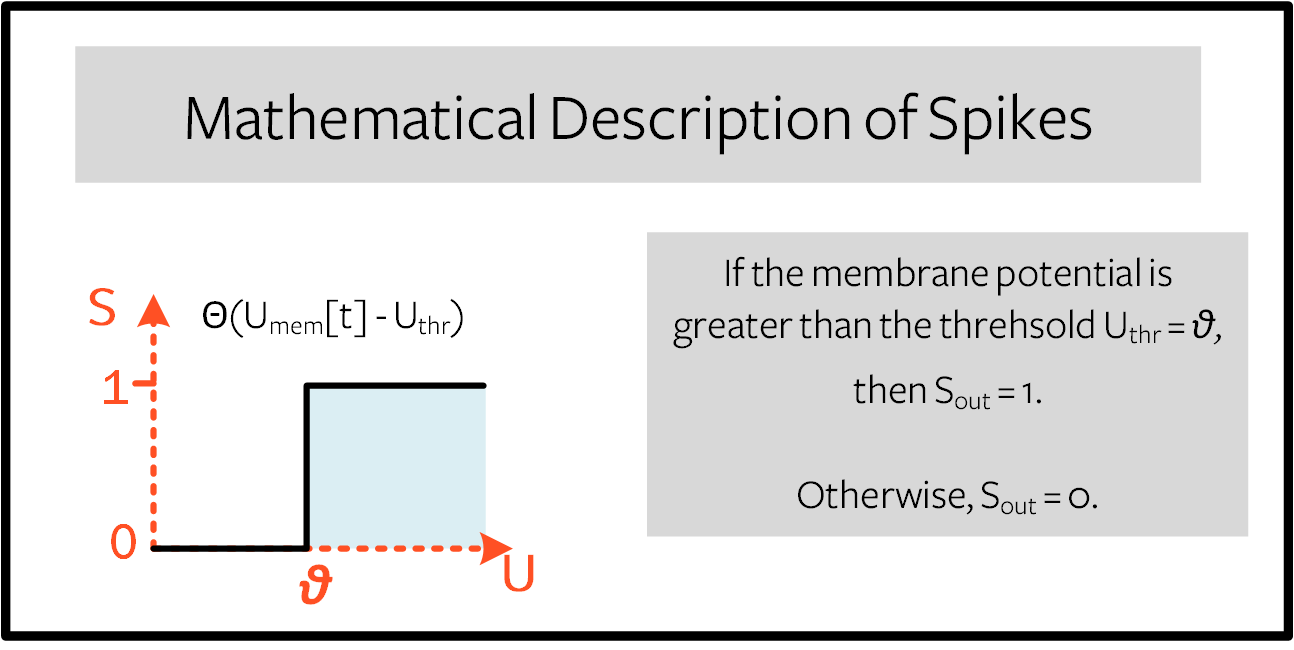
\includegraphics[scale=1.4]{spike_descrip.png}}
\label{ris:spike_descrip}
\end{figure}

Основная проблема в обучении спайковых нейронных сетей в том, что при обучении один из элементов производной функции потерь равен или 0, или бесконечности, что не дает нам обучаться.

\begin{figure}[!h]
\center{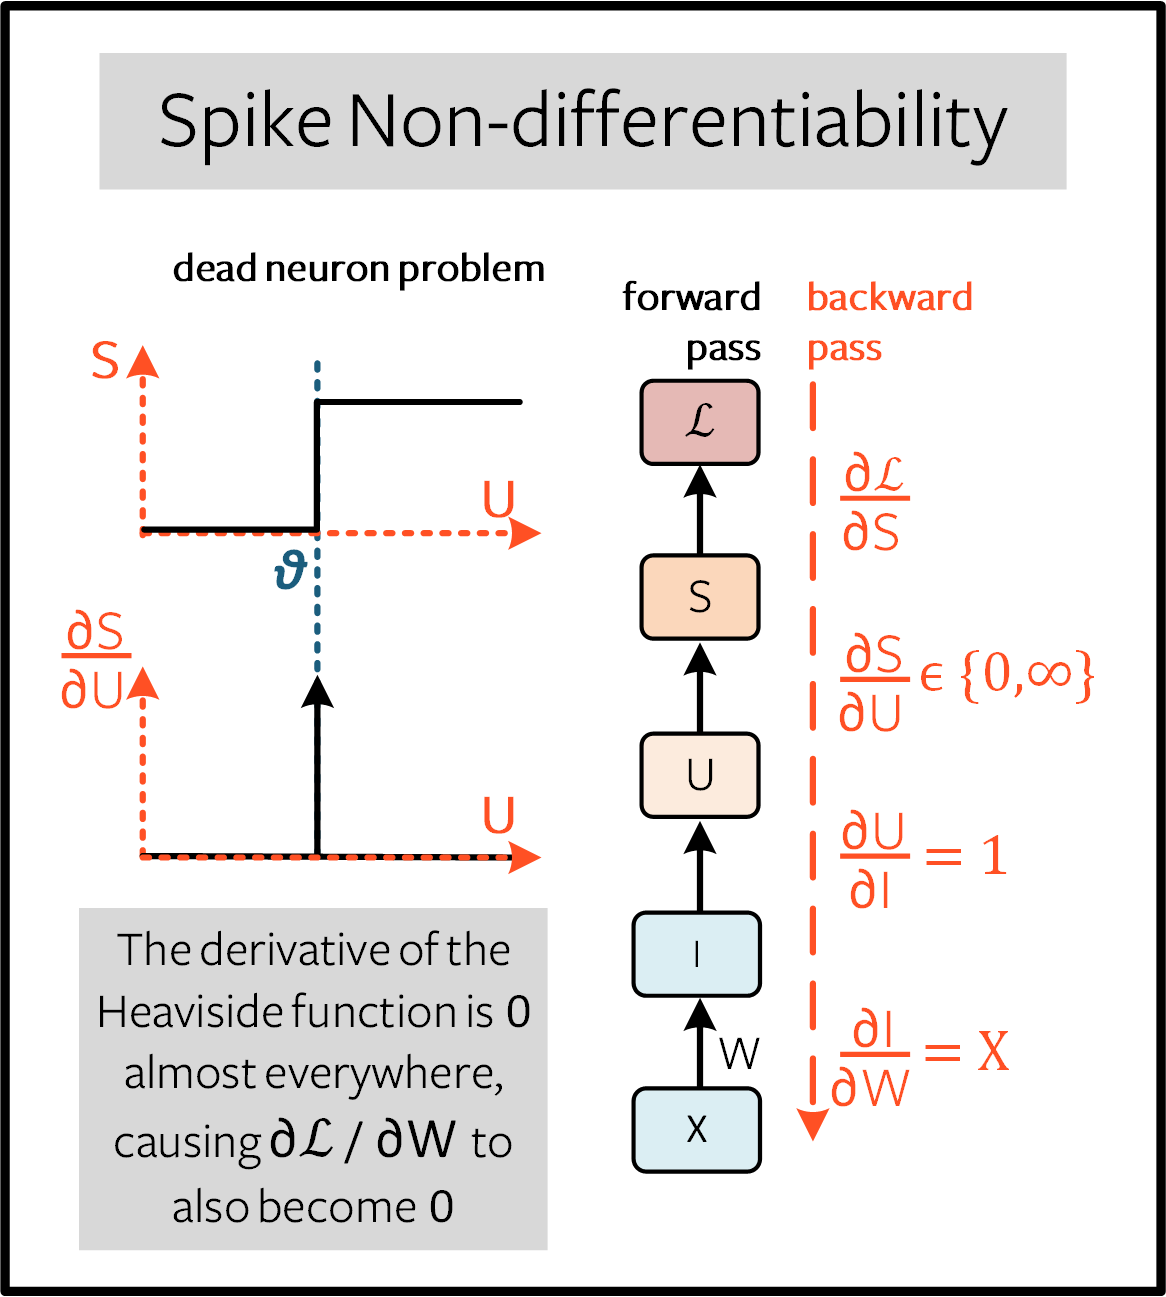
\includegraphics[scale=0.8]{non-diff.png}}
\label{ris:spike_descrip}
\end{figure}

\newpage

В качестве решения данной проблемы возможно приравнять производную к самой функции:

$$ \frac{\partial \tilde{S}}{\partial U} \leftarrow S = \begin{cases} 1, &\text{if}~U> U_{thr} \\
0, &\text{otherwise}\end{cases} $$

Другим вариантов является аппроксимация функции Хэвисайда:

$$
    \tilde{S} = \frac{U_{OD}}{1+k|U_{OD}|},\\
    \frac{\partial \tilde{S}}{\partial U} = \frac{1}{(k|U_{OD}|+1)^2},\\
    \frac{\partial \tilde{S}}{\partial U} = \frac{1}{(k|U_{OD}|+1)^2}
$$

\begin{figure}[!h]
\center{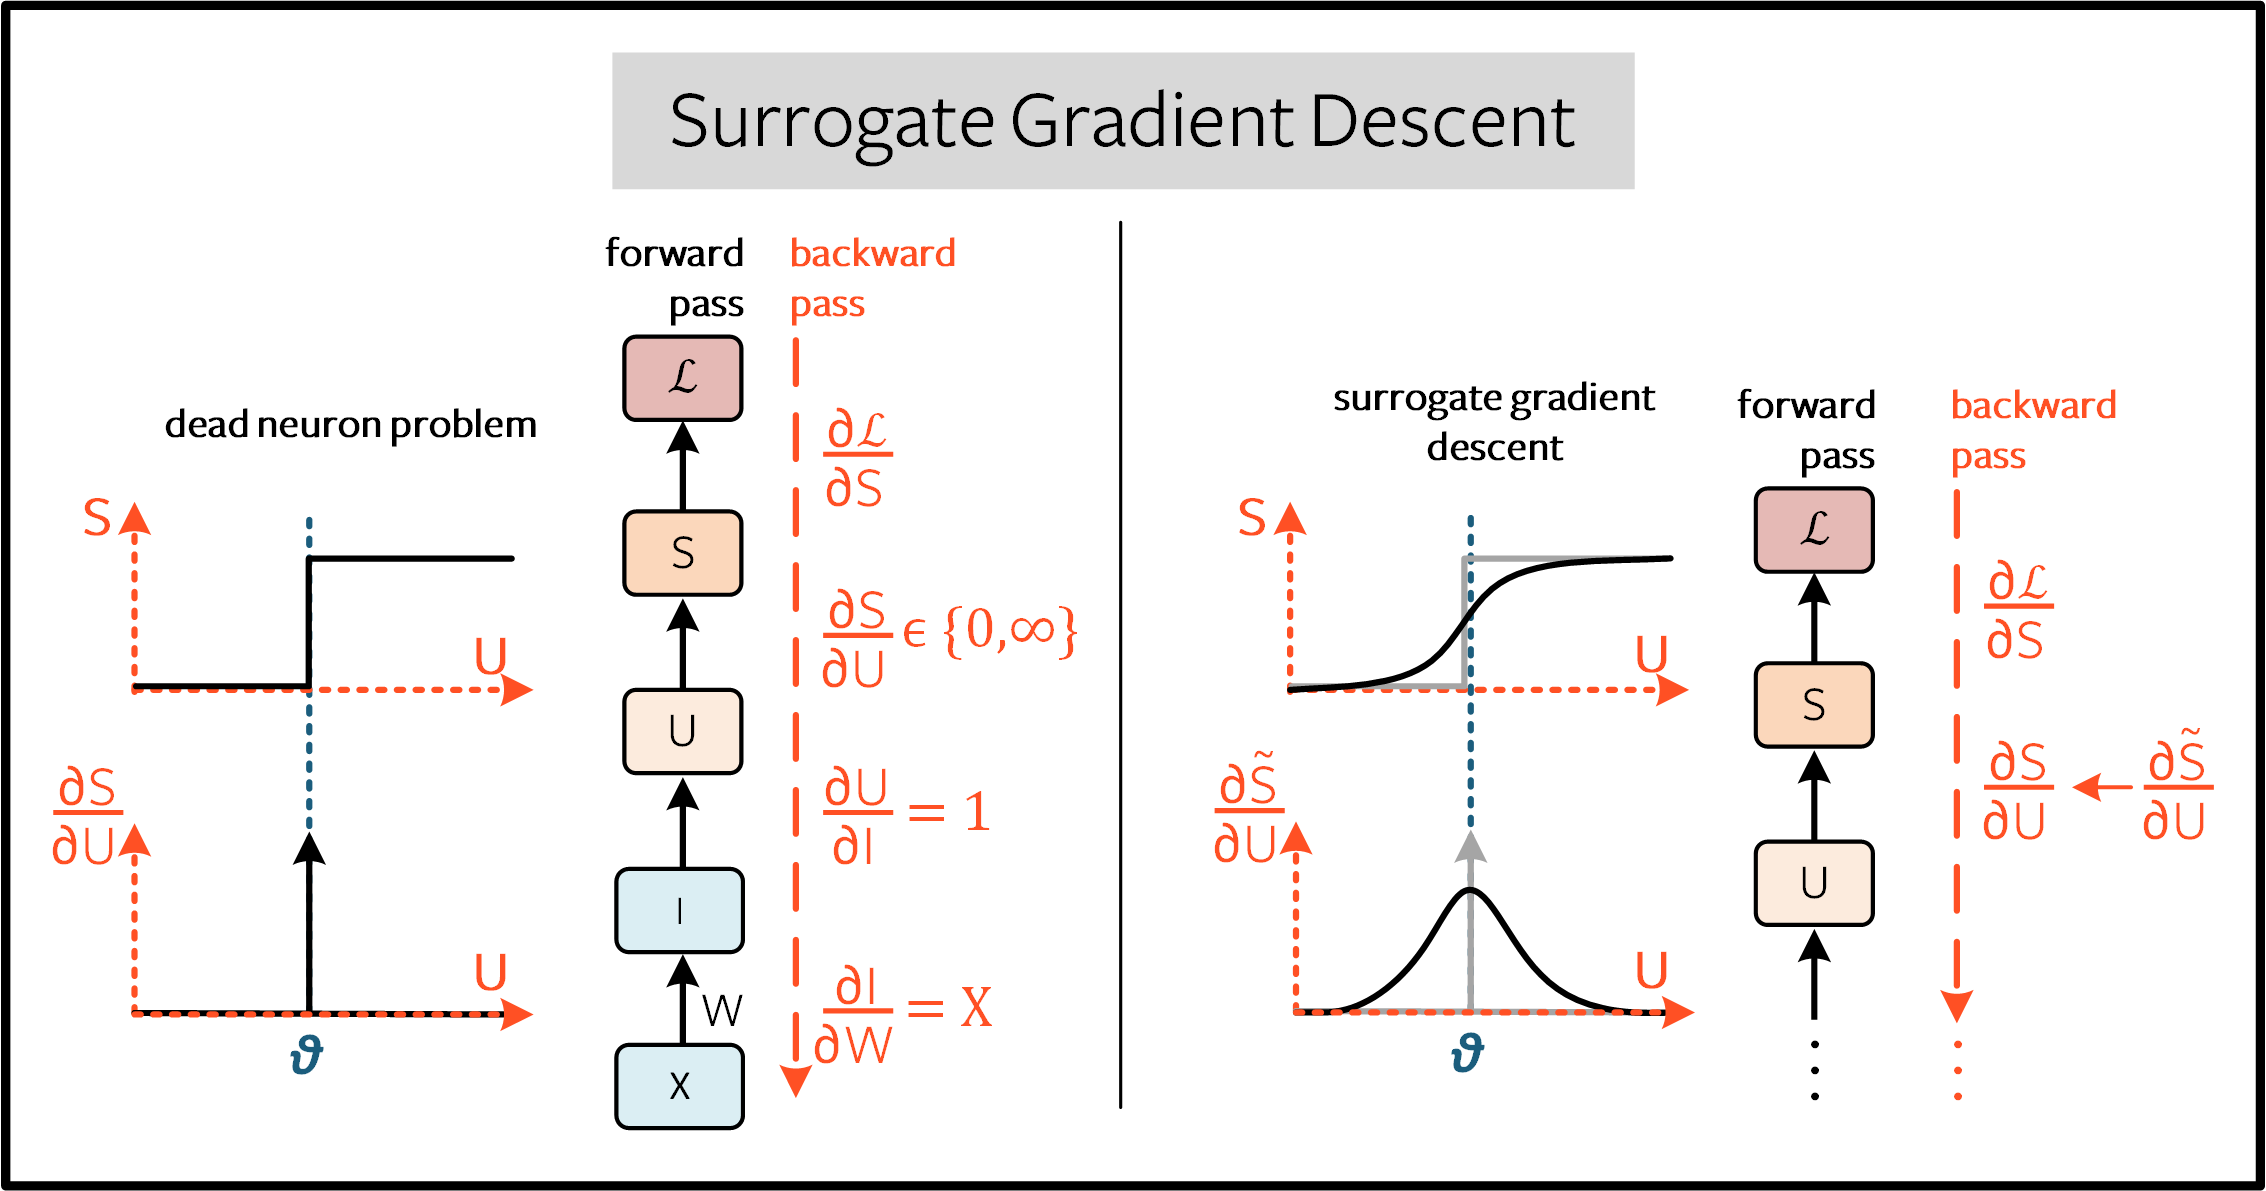
\includegraphics[scale=0.7]{surrogate.png}}
\label{ris:spike_descrip}
\end{figure}

\newpage

\section{Результаты экспериментов}

\subsection{Синусоидальные данные}

Для начала полносвязная и рекуррентная сети были обучены предсказывать направление дальнейшего движения графиков функций $sin(x)$ и $0.5sin(x) + 0.5sin(6x) + 1$.

\begin{figure}[!h]
\center{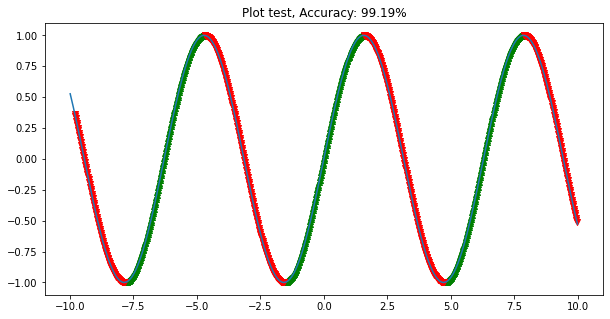
\includegraphics[scale=0.7]{sinx.png}}
\caption{Предсказаие SLSTM}\label{ris:sinx}
\end{figure}

\begin{figure}[!h]
\center{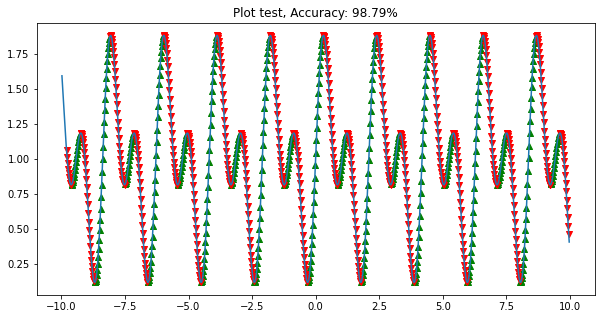
\includegraphics[scale=0.7]{sin3x.png}}
\caption{Предсказаие SLSTM}\label{ris:sin3x}
\end{figure}

\subsection{Синусоидальные данные с трендом}

После этого нейросети научились предсказывать направление движения графиков этих же функций, но с трендом. 

Можно отметить, что полносвязной сети не хватило 50 эпох для обучения на функции $sin(x)$ с трендом, в отличие от сети SLSTM. 

\begin{figure}[!h]
\center{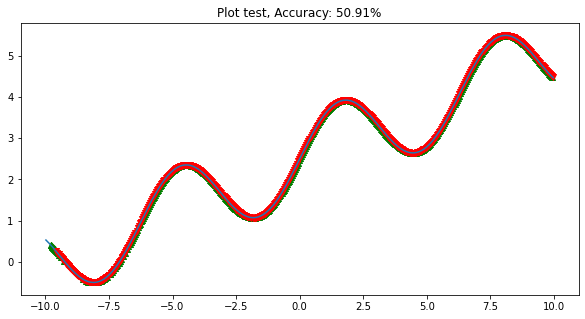
\includegraphics[scale=0.7]{sinx_trend.png}}
\caption{Предсказаие полносвязной сети, обученной за 50 эпох}\label{ris:sinx_trend}
\end{figure}

\begin{figure}[!h]
\center{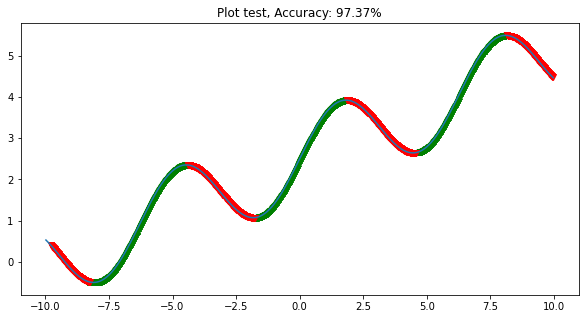
\includegraphics[scale=0.7]{sinx_trend_slstm.png}}
\caption{Предсказаие SLSTM, обученной за 50 эпох}\label{ris:sinx_trend}
\end{figure}

Аналогичная ситуация и с функцией $0.5sin(x) + 0.5sin(6x) + 1$.

\begin{figure}[!h]
\center{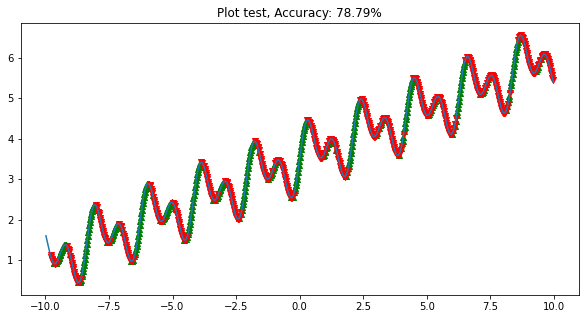
\includegraphics[scale=0.7]{sin3x_trend.png}}
\caption{Предсказаие полносвязной сети, обученной за 50 эпох}\label{ris:sin3x_trend}
\end{figure}

\begin{figure}[!h]
\center{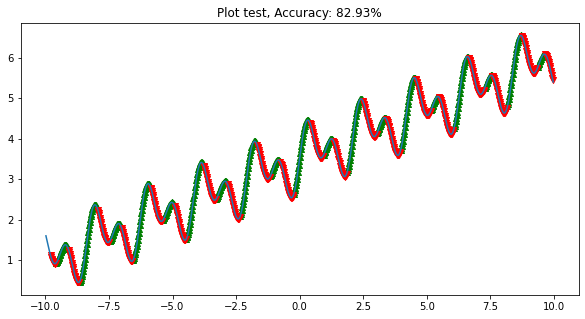
\includegraphics[scale=0.7]{sin3x_trend_slstm.png}}
\caption{Предсказаие SLSTM, обученной за 50 эпох}\label{ris:sinx_trend}
\end{figure}

Это показывает, что рекуррентные сети лучше работают с запоминанием последовательностей.

\subsection{Направление движения цены акции}

Далее сеть SLSTM была обучена для предсказания направления движения цены акции. В качестве данных для обучения были взяты цены акции из банковского сектора российского рынка за 2020-2021 год. В качестве тестовых данных - цены этой же акции за 2021-2022 год.

\begin{figure}[!h]
\center{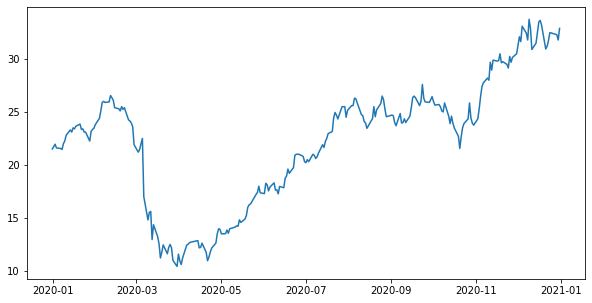
\includegraphics[scale=0.7]{stock.png}}
\caption{Цена одной акции за период с 01.01.2020 по 01.01.2021}\label{ris:sinx_trend}
\end{figure}

Обучение на данных цены не увенчалось успехом, поэтому было произведено обучение на данных технического индикатора MACD, построенного на графике цен акции.

Во время обучения были проверены различные комбинации гиперпараметров и было проведено около 500 экспериментов.

\begin{itemize}
    \item Модели: полносвязная, SLSTM;
    \item Размер скрытого слоя: 8, 16, 32;
    \item Порог активации нейронов: 0.1, 0.2, 0.3, 0.4, 0.5;
    \item Обучение порога: да, нет;
    \item Механизм <<сброса>>: вычитание, сброс до 0, без сброса;
    \item коэффициент beta: 0.5, 0.6, 0.7, 0.8, 0.9.
\end{itemize}

\begin{figure}[!h]
\center{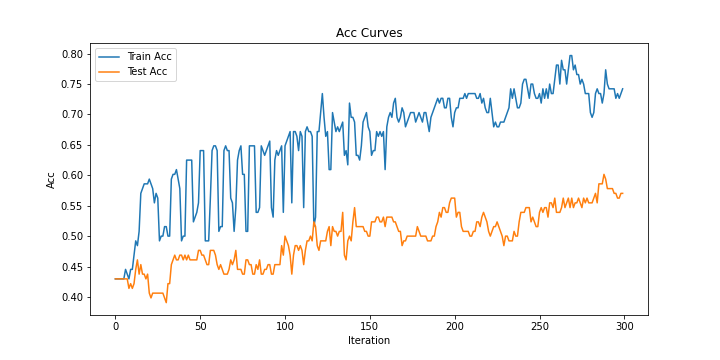
\includegraphics[scale=0.6]{acc.png}}
\caption{Значения accuracy во время обучения}\label{ris:sinx_trend}
\end{figure}

\begin{figure}[!h]
\center{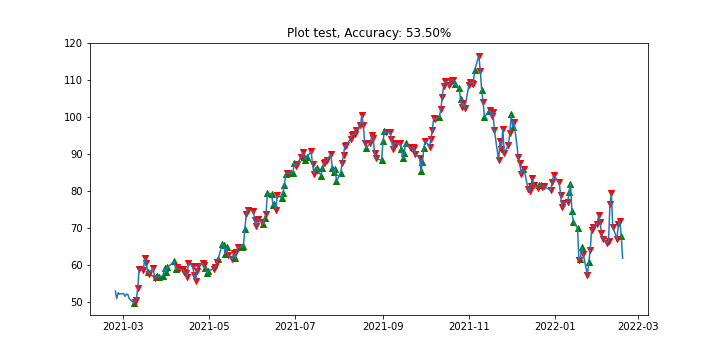
\includegraphics[scale=0.6]{res.png}}
\caption{Предсказания сети на тестовых данных}\label{ris:sinx_trend}
\end{figure}

Лучшие результаты обучения показаны ниже. К сожалению, лучшая модель показала итоговое значение accuracy 58.59\% на тестовых данных и 80\% на данных для обучения. 

Для сравнения были написаны две простые стратегии: случайная и упрощенное правило <<моментов>>, то есть если стоимость акции выросла за последний временной промежуток, то она будет расти и дальше. 

Случайная стратегия давала результаты 46-51\%.

Стратегия правила <<моментов>> - 51.5\%.

То есть, обученная сеть работает лучше упомянутых выше правил, но, тем не менее, результаты все еще далеки от идеала.

Параметры лучшей модели:

\begin{itemize}
    \item Размер скрытого слоя: 16;
    \item Порог активации нейронов: 0.1;
    \item Механизм <<сброса>>: сброс до 0;
    \item Без обучения порога активации;
\end{itemize}

\section{Направление дальнейших исследований}

В качестве направлений для дальнейших исследований в данной области и возможных улучшений предлагается следующее:

\begin{itemize}
    \item Улучшение архитектуры сети:
    Возможно использование комбинации SLSTM и линейных слоев и другие эксперименты;
    \item Борьба с переобучением;
    \item Новые признаки:
    Исползование различных индикаторов технического анализа (в том числе RSI) и их комбинаций;
    \item Признаки в виде спайков:
    Описать признаковое пространство в виде последовательности спайков;
    \item Обучение биологическими методами:
    Применить биологический подход к обучению, например, с помощью STDP.
\end{itemize}

\section{Выводы}

\begin{itemize}
    \item Были изучены спайковые нейронные сети, в том числе рекуррентные, и градиентные методы их обучения
    \item Были изучены спайковые нейронные сети, в том числе рекуррентные, и градиентные методы их обучения;
    \item Спайковые сети были обучены для предсказания направления движения синусоидальных функций;
    \item Рекуррентные сети обучаются лучше и быстрее, по крайней мере на простых данных;
    \item Спайковые сети были обучены для предсказания направления движения цены акции;
    мРезультаты работы сети на тестовых данных оказались лучше «случайного» выбора и упрощенного правила «моментов», но все равно далеки от идеала;
    \item Для достижения более качественных результатов предсказания необходимы дальнейшие исследования.
\end{itemize}

\addcontentsline{toc}{section}{Список используемой литературы}

\begin{thebibliography}{}

\bibitem{techan}
Эрлих А. А. Технический анализ товарных и финансовых рынков: Прикладное пособие. 2-е изд. М.: ИНФРА-М, 1996. 176 с.

\bibitem{snntorch}
Документация библиотеки snnTorch. - [Электронный ресурс]. - Электрон. дан. - URL: https://snntorch.readthedocs.io/en/latest/ (дата обращения 15.07.2022).

\bibitem{snntraining}
Jason K. Eshraghian, Max Ward, Emre Neftci, Xinxin Wang, Gregor Lenz, Girish Dwivedi, Mohammed Bennamoun, Doo Seok Jeong, and Wei D. Lu. <<Training Spiking Neural Networks Using Lessons From Deep Learning>>. arXiv preprint arXiv:2109.12894, September 2021.

\bibitem{lstm}
Sepp Hochreiter and Jurgen Schmidhuber. Long Short-Term Memory. Neural Computation 9.8, 1997, pp. 1735–1780. DOI: 10.1162/neco.1997.9.8.1735.

\end{thebibliography}

\end{document}
